\section{Experiments}
\label{sec:gmm-experiments}
While \cref{subsec:fg-conservation,sec:gmm-gmm,sec:gmm-hypotheses} elaborated on the conservation
tracking model and its theoretical background, this section is dedicated to the performance of the
conservation tracking model on data and experimental results. To this end, we first provide a
summary of the implementation details in \cref{subsec:gmm-impl}, followed by a short presentation of
the data used for experiments in \cref{subsec:gmm-data}. Then, \cref{subsec:gmm-measures} introduces
the measures which are used for the evaluation of experimental results in \cref{subsec:gmm-results}.


\subsection{Implementation}
\label{subsec:gmm-impl}
In the context of implementation, methods that infer a labeling of the hypotheses graph are called
\emph{reasoners}~\citep[15]{kausler_13_tracking}. The C++ library
\emph{pgmlink}\footnote{\url{https://github.com/bekaus/pgmlink}\nocite{kausler_12_pgmlink}}~\citep[Chapter~6.1]{kausler_13_tracking}
provides a tracking-by-assignment framework with a hypotheses graph data structure
\emph{HypothesesGraph}, based on the C++ graph library \emph{lemon}\footnote{\url{http://lemon.cs.elte.hu/trac/lemon}}~\citep{dezso_11_lemon}, and an abstract
class \emph{Reasoner} as an interface for modeling a reasoner method. In this context, the
conservation tracking method is implemented as an extension of the pgmlink library by providing a
subclass of the Reasoner class~\citep{schiegg_13_conservation}, \emph{ConservationTracking}, and by
integrating the \emph{GMM} class of the machine learning library \emph{mlpack}~\citep{mlpack2013},
for cell identity reconstruction~(our contribution). In general, the pgmlink library uses
\emph{opengm}\footnote{\url{http://hci.iwr.uni-heidelberg.de/opengm2/}}~\citep{andres_12_opengm} for
modeling the factor graph and as an interface to \emph{ILOG
    CPLEX}\footnote{\url{http://www.ilog.com/products/cplex}} for inference.

An interface for the high-level language \emph{Python}\footnote{\url{http://www.python.org}} is provided
for integration of the conservation tracking into the \emph{Interactive Learning and Segmentation
    Toolkit}~\citep{sommer_11_ilastik}, which, moreover, \citet{schiegg_13_conservation} use for
segmenting the raw data and training the random forest classifiers for cell
divisions~(\cref{eq:fg-conservation-div}) and connected component
size~(Equations \ref{eq:fg-conservation-det-a}-\ref{eq:fg-conservation-det-c} on \pageref{eq:fg-conservation-det-c}). Both the segmentation
and classifier training make use of the random forest class provided by the \emph{Vision with
    Generic Algorithms}
library\footnote{\url{http://hci.iwr.uni-heidelberg.de/vigra}}~(vigra,~\citealp{koethe_08_vigra}).

In summary, the conservation tracking pipeline consists of the following steps:
\begin{enumerate}
      \item Segment the raw data into foreground and cell candidates.
      \item Train random forest classifiers for divisions and connected component size.
      \item Set up model parameters $w_{\text{app}}$, $w_{\text{dis}}$, $m$ and $p$ \cref{subsec:fg-conservation} and run the tracking algorithm.
\end{enumerate}

\subsection{Data}
\label{subsec:gmm-data}
\citet{schiegg_13_conservation} choose three challenging data sets for the evaluation of their
method. Their selection contains two $3d+t$ data sets A and B, and one $2d+t$ data set C. In the
following, each of these data sets is presented. A summary of their characteristics can be found in
\cref{tab:gmm-evaluation-data}.

\subsubsection{Data Set A -  Drosophila Embryo in Syncytial Blastoderm}
The first data set is a time series of volumes of size $2362\times994\times47$ over 40 time
steps~\citep[43]{kausler_13_tracking}, each containing about 300 cells on average, with a dynamic
intensity range of 8 bits and a physical resolution of \SI{0.1625}{\micro\metre} (lateral) and
\SI{2}{\micro\metre} (axial). The recording shows an
autofluorescent~\citep{mavrakis_08_fluorescence} fruit fly (drosophila) in \emph{syncytial
    blastoderm} which is formed about one and a half hours after fertilization and lasts about 90
minutes. In this phase, the cell nuclei form a syncytium -- a common cytoplasm shared between nuclei
without separating membranes -- and inhabit the outer rim of the cigar shaped embryo and have no
separating membranes. A more detailed explanation can be found in \citet{wolpert_07_principles}.

An excerpt of the data is shown in \cref{fig:gmm-data-a} on Page~\pageref{fig:gmm-data-a}. Data has been
acquired by the lab of Lars Hufnagel at the European Molecular Biology Laboratory (EMBL) in
Heidelberg in fall 2011 with an in-house developed light sheet
microscope~\citep{krzic_12_multiview}.  This data set is made challenging by the radiance of the
cytoplasm, which produces a large number of false positive detections in the
segmentation~(\cref{fig:gmm-data-a-false-positive}).

\begin{figure}
    \centering
    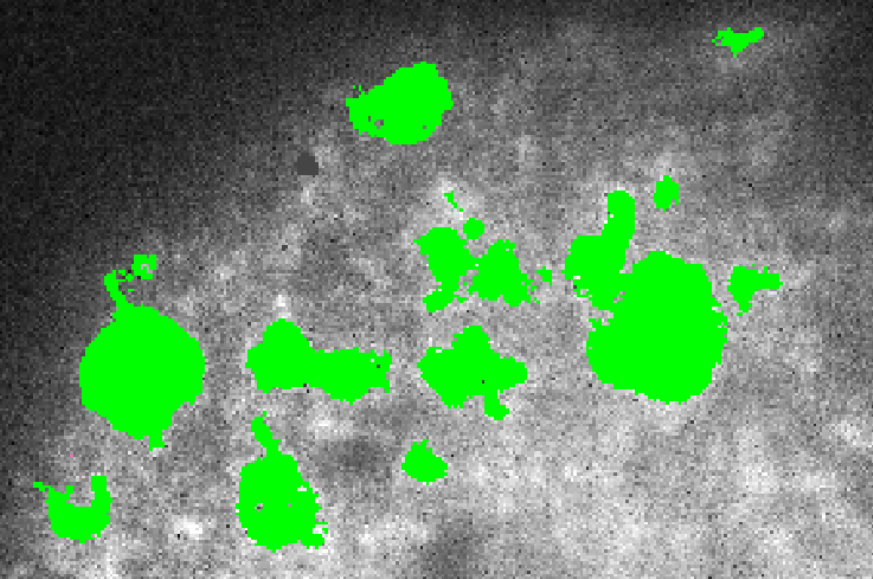
\includegraphics[width=0.7\textwidth]{images/gmm/data/A/dataA_false_positive.png}
    \caption[An excerpt of data set A - detections]{An excerpt of data set A
        (taken from~\citet{schiegg_13_conservation}): Detections are indicated by green color. A high
        false positive rate makes this data set challenging.}
    \label{fig:gmm-data-a-false-positive}
\end{figure}



\subsubsection{Data Set B - Drosophila Embryo past Gastrulation}
The second three-dimensional data set is another $3d+t$ recording of drosophila, but this time from
a later stage in the development of the embryo -- shortly after gastrulation. It is a time series of
100 volumes of the size $730 \times 320 \times 30$ with about 800 cells per frame. Due to the
advanced embryonic evolution, the cell population is much denser compared to data set
A~(\cref{fig:gmm-data-b-dense-population}). This increases the number of merged objects in the
segmentation~(\cref{fig:gmm-result-b} on Page~\pageref{fig:gmm-data-b-dense-population}) and therefore is
a demanding challenge fit to the capabilities of the conservation tracking.


\subsubsection{Data Set C - MitoCheck}
\label{subsubsec:gmm-data-c}
Finally, the third data set is a series of 92 $2d$ images with a resolution of $1344\times1024$,
publicly available on the website of the MitoCheck
project\footnote{\label{note1}\url{http://www.mitocheck.org/archive/cgi-bin/mtc?action=show_movie;query=87214}}. Due
to its two-dimensional nature, it contains merged objects caused not only by poor image quality but
also by occlusions. \cref{fig:gmm-data-c-three-slices} on Page~\pageref{fig:gmm-data-c-three-slices}
shows three frames of the data with an increasing number of cells and merged objects.





\begin{table}
    \centering
    \begin{tabularx}{\textwidth}{Xp{2cm}XX}
        \toprule
        Data set & Dimensions & Resolution & Challenge \\ \midrule
        A - Syncytial Blastoderm & $3d+t$ &  $40\times2362\times994\times47$& High false positive
        detection rate
        due to cytoplasm radiance \\
        B - Gastrulation & $3d+t$ & $100 \times 730 \times 320 \times 30$ & Many merged objects \\
        C - MitoCheck & $2d+t$ & $92\times1344\times1024$ & Many merged objects \\
        \bottomrule
    \end{tabularx}
    \caption[Data sets for evaluation of the conservation tracking]{Data sets for evaluation of the
        conservation tracking.}
    \label{tab:gmm-evaluation-data}
\end{table}

\subsection{Measures}
\label{subsec:gmm-measures}
In general, a tracking method is compared to ground truth for evaluation. Based on the \emph{true
    positive} events, \ie these events appear both in the experiment and ground truth, and the
\emph{false positive} and \emph{false negative} events, \ie these events appear in the experiment,
but not in the ground truth, and vice versa, we can define the performance measures
\emph{precision}, \emph{recall} and
\emph{$\fscore_\beta$-score}~\citep{powers_07_evaluation,makhoul_99_performance}. In the
following, $\tp$, $\fp$ and $\fn$ denote the numbers of true positives, false positives and false
negatives, respectively. Then, those three measures can be defined as
\begin{align}
    \precision &= \frac{\tp}{\tp+\fp} \in [0,1], \\
    \recall &= \frac{\tp}{\tp+\fn} \in [0,1], \\
    \fscore_\beta &= \left(1+\beta^2\right)\frac{\precision\cdot\recall}{\beta^2\precision+\recall} \in [0,1].
\end{align}
In a more descriptive way, precision and recall are the fractions of events in the experimental
results and ground truth, respectively, which were classified correctly. The weight $\beta$ in the
$\fscore_\beta$-score indicates the relative cost of false positives and false
negatives. Furthermore, with the commonly used setting $\beta=1$,
\begin{align}
    \fmeasure = 2\frac{\precision\cdot\recall}{\precision+\recall}
\end{align}
is the harmonic mean of precision and recall and indicates equal costs for Type-I and Type-II
errors. Naturally, a higher value of these measures reflects a better performance of a method. In
general, we set $\beta=1$ and use precision, recall and $\fmeasure$ for the evaluation of the
different event types listed in \cref{tab:gmm-events}.
\begin{table}
    \centering
    \begin{tabularx}{\textwidth}{lXl}
        \toprule
        \multicolumn{3}{l}{Event}  \\ \midrule
        Move & Cell $i$ at time $t$ is assigned to cell $j$ at time $t+1$. &
        \tikz[baseline=(t1.south),minimum size=58pt,scale=0.35, every node/.style={scale=0.35,
            text=black, font=\LARGE}, thick]{
            \begin{scope}
    \node (t1) {\huge $t$};
    \node[hypotheses_one_object, below=of t1.north, circle, draw,yshift=10mm] (x11) {$X_i^t$};
\end{scope}

\begin{scope}
    \node[right=of t1, xshift=-10mm] (t2) {\huge $t+1$};
    \node[hypotheses_one_object, below=of t2.north, circle, draw,yshift=10mm] (x21) {$X_j^{t+1}$};
\end{scope}

\path[hypothesestransition] (x11) edge (x21);

\begin{scope}[on background layer]
    \node[rectangle, draw, color=hypothesesbackground!40, fill=hypothesesbackground!30,
    fit=(x11), inner sep=4mm] (b1) {};
    \node[rectangle, draw, color=hypothesesbackground!40, fill=hypothesesbackground!30,
    fit=(x21), inner sep=4mm] (b2) {};
\end{scope}

%%% Local Variables: 
%%% mode: latex
%%% TeX-master: "../../../main"
%%% End: 

        }\\
        Division & Cell $i$ at time $t$ divides into cells $j$ and $h$ at time $t+1$. &
        \tikz[baseline=(t1.south),minimum size=58pt,scale=0.35, every node/.style={scale=0.35,
            text=black, font=\LARGE}, thick]{
            \begin{scope}
    \node (t1) {\huge $t$};
    \node[hypotheses_one_object, below=of t1.north, circle, draw,yshift=-2mm] (x11) {$X_i^t$};
\end{scope}

\begin{scope}[on background layer]
    \node[hypotheses_one_object, below=of t1.north, circle, draw,yshift=10mm] (x12) {$X_j^{t+1}$};
    \node[hypotheses_one_object, below=of t1.north, circle, draw,yshift=-21mm] (x13) {$X_h^{t+1}$};
\end{scope}

\begin{scope}
    \node[right=of t1, xshift=-10mm] (t2) {\huge $t+1$};
    \node[hypotheses_one_object, below=of t2.north, circle, draw,yshift=10mm] (x21) {$X_j^{t+1}$};
    \node[hypotheses_one_object, hypothesesdetection, below=of t2.north, circle, draw,yshift=-21mm] (x22) {$X_h^{t+1}$};
\end{scope}

\path[hypothesestransition] (x11) edge (x21);
\path[hypothesestransition] (x11) edge (x22);

\begin{scope}[on background layer]
    \node[rectangle, draw, color=hypothesesbackground!40, fill=hypothesesbackground!30,
    fit=(x12) (x13), inner sep=4mm] (b1) {};
    \node[rectangle, draw, color=hypothesesbackground!40, fill=hypothesesbackground!30,
    fit=(x21) (x22), inner sep=4mm] (b2) {};
\end{scope}


%%% Local Variables: 
%%% mode: latex
%%% TeX-master: "../../../main"
%%% End: 

        }\\
        Merger & Connected component $i$ at time $t+1$ is identified to be a merger of size $k$. In the example in
        the right column $k=2$.&
        \tikz[baseline=(t1.south),minimum size=58pt,scale=0.35, every node/.style={scale=0.35,
            text=black, font=\LARGE}, thick]{
            \begin{scope}
    \node (t2) {\huge $t$};
    \node[hypotheses_one_object, below=of t2.north, circle, draw,yshift=10mm] (x21) {$X_i^{t}$};
    \node[hypotheses_one_object, below=of t2.north, circle, draw,yshift=-21mm] (x22) {$X_h^{t}$};
\end{scope}

\begin{scope}
    \node[right=of t2, xshift=-10mm] (t1) {\huge $t+1$};
    \node[hypotheses_two_objects, below=of t1.north, circle, draw,yshift=-2mm] (x11) {$X_i^{t+1}$};
\end{scope}

\begin{scope}[on background layer]
    \node[hypothesesdetection, below=of t1.north, circle, draw,yshift=10mm] (x12) {$X_j^{t+1}$};
    \node[hypothesesdetection, below=of t1.north, circle, draw,yshift=-21mm] (x13) {$X_h^{t+1}$};
\end{scope}



\path[hypothesestransition] (x11) edge (x21);
\path[hypothesestransition] (x11) edge (x22);

\begin{scope}[on background layer]
    \node[rectangle, draw, color=hypothesesbackground!40, fill=hypothesesbackground!30,
    fit=(x12) (x13), inner sep=4mm] (b1) {};
    \node[rectangle, draw, color=hypothesesbackground!40, fill=hypothesesbackground!30,
    fit=(x21) (x22), inner sep=4mm] (b2) {};
\end{scope}


%%% Local Variables: 
%%% mode: latex
%%% TeX-master: "../../../main"
%%% End: 

        }\\
        Multiframe Move & Cell $i$ at time $t$ moves into a merged object at time $t+1$ and is
        identified as a single cell $j$ at time $t^{\prime}>t+1$.  &
        \tikz[baseline=(t1.south),minimum size=58pt,scale=0.35, every node/.style={scale=0.35,
            text=black, font=\LARGE}, thick]{
            \begin{scope}
    \node (t2) {\huge $t$};
    \node[hypotheses_one_object, below=of t2.north, circle, draw,yshift=10mm] (x21) {$X_l^{t}$};
    \node[hypotheses_one_object, below=of t2.north, circle, draw,yshift=-21mm] (x22) {$X_h^{t}$};
\end{scope}

\begin{scope}
    \node[right=of t2, xshift=-10mm] (t1) {\huge $t+1$};
    \node[hypotheses_two_objects, below=of t1.north, circle, draw,yshift=-2mm] (x11) {$X_i^{t+1}$};
\end{scope}

\begin{scope}[on background layer]
    \node[hypotheses_one_object, below=of t1.north, circle, draw,yshift=10mm] (x12) {$X_j^{t+1}$};
    \node[hypotheses_one_object, below=of t1.north, circle, draw,yshift=-21mm] (x13) {$X_h^{t+1}$};
\end{scope}

\begin{scope}
    \node[right=of t1, xshift=10mm] (t3) {\huge $t^{\prime}-1$};
    \node[hypotheses_two_objects, below=of t3.north, circle, draw,yshift=-2mm] (x31) {$X_m^{t^{\prime}-1}$};
\end{scope}

\begin{scope}[on background layer]
    \node[hypotheses_one_object, below=of t3.north, circle, draw,yshift=10mm] (x32) {$X_j^{t}$};
    \node[hypotheses_one_object, below=of t3.north, circle, draw,yshift=-21mm] (x33) {$X_h^{t+1}$};
\end{scope}

\begin{scope}
    \node[right=of t3, xshift=-10mm] (t4) {\huge $t^{\prime}$};
    \node[hypotheses_one_object, below=of t4.north, circle, draw,yshift=10mm] (x41) {$X_n^{t^{\prime}}$};
    \node[hypotheses_one_object, below=of t4.north, circle, draw,yshift=-21mm] (x42) {$X_j^{t^{\prime}}$};
\end{scope}

% \coordinate[xshift=8mm] at (x11.east) (c1);
% \coordinate[xshift=-8mm] at (x31.west) (c2);



\path[hypothesestransition] (x11) edge (x21);
\path[hypothesestransition] (x11) edge (x22);
\path[hypothesestransition] (x31) edge (x41);
\path[hypothesestransition] (x31) edge (x42);
\path[hypothesestransition, dashed] ($(x11.east)!0.2!(x31.west)$) edge ($(x11.east)!0.8!(x31.west)$);

\begin{scope}[on background layer]
    \node[rectangle, draw, color=hypothesesbackground!40, fill=hypothesesbackground!30,
    fit=(x12) (x13), inner sep=4mm] (b1) {};
    \node[rectangle, draw, color=hypothesesbackground!40, fill=hypothesesbackground!30,
    fit=(x21) (x22), inner sep=4mm] (b2) {};
    \node[rectangle, draw, color=hypothesesbackground!40, fill=hypothesesbackground!30,
    fit=(x32) (x33), inner sep=4mm] (b2) {};
    \node[rectangle, draw, color=hypothesesbackground!40, fill=hypothesesbackground!30,
    fit=(x41) (x42), inner sep=4mm] (b1) {};
\end{scope}


%%% Local Variables: 
%%% mode: latex
%%% TeX-master: "../../../main"
%%% End: 

        }\\ \bottomrule
    \end{tabularx}

%%% Local Variables: 
%%% mode: latex
%%% TeX-master: "../../../main"
%%% End: 

    \caption[Events in the conservation tracking]{Events for evaluation in the conservation tracking
        experiment. Note that a correct classification of a division requires not only that the
        parent cell is detected, but also the correct child cells. Furthermore, a merger event is
        only classified correctly if the correct number of objects has been inferred.}
    \label{tab:gmm-events}
\end{table}

\subsection{Results}
\label{subsec:gmm-results}
In this section we evaluate the performance of our proposed method on the data sets presented in
\cref{subsec:gmm-data}. Based on the measures defined in \cref{subsec:gmm-measures} we compare our
method to the state of the art tracking-by-assignment algorithm by \citet{kausler_12_discrete}.  In
addition to the evaluation of the tracking, we show the stand-alone performance of the division and
cell classifiers, where applicable. For the division classifier evaluation, contrary to the
evaluation of divisions in the tracking result, the correct classification of a mitotic cell, \ie a
cell that will divide in the subsequent time step, is sufficient.


\begin{table}
    \centering\small
    \begin{tabularx}{\textwidth}{c||c|cccc|cccc}
        \toprule
        & A & \multicolumn{4}{c|}{B} &
        \multicolumn{4}{c}{C} \\ 
        Parameter& $m=1$ & $m=1$ & $m=2$ & $m=3$ & $m=4$ & $m=1$ & $m=2$ & $m=3$ & $m=4$\\ \hline\small
        $\alpha$ & $25$ &5&5&5&5&5&5&5&5\\
        $w_{\text{app}}$ & $50$ &50&100&100&100&100&100&100&100\\
        $w_{\text{dis}}$ & $50$ &100&100&100&100&100&100&100&100\\
        $w_{\text{tr}}$ & $13$ &33&22&22&24&10&10&10&10\\
        $w_{\text{div}}$ & $28$ &40&26&41&36&36&16&16&16\\
        \bottomrule
    \end{tabularx}
    \caption[Conservation tracking - parameter settings]{Parameter settings for the conservation
        tracking in the experiments for data sets A, B and C~(\cref{subsec:gmm-data}). In all cases,
    the parameters were determined in an exhaustive grid search.}
    \label{tab:gmm-experiments-parameters}
\end{table}

\subsubsection{Data Set A -  Drosophila Embryo in Syncytial Blastoderm}
\label{subsubsec:gmm-reults-data-a}
For the comparison of the methods on data set A, we apply both tracking algorithms to a published
segmentation. This segmentation contains many false positive detections due to noise and
no merged objects~(\cref{fig:gmm-data-a-false-positive}). Therefore, we set the maximum number of
objects per connected component, model parameter $m$, to one. Furthermore, we use the same
classifier for detected cell as \citet{kausler_12_discrete}.

We obtain the optimal parameter settings~(\cref{tab:gmm-experiments-parameters}) in a grid
search. The tracking results are then evaluated based on precision, recall and
$\fmeasure$~(\cref{tab:gmm-experiments-data-a-results}). Our method yields comparable results
($\fmeasure=0.94$ and $\fmeasure=0.90$ on moves and divisions respectively) with
\citet{kausler_12_discrete} performing marginally better ($\fmeasure=0.96$ for moves and
$\fmeasure=0.92$ for divisions). The slightly better performance of \citet{kausler_12_discrete} can
be explained by their exploitation of the cell cycle
duration~\citep[Figure~5b]{kausler_12_discrete}.

\begin{table}
\centering
% \scalebox{0.8} {
\begin{tabular}{l||ccc|ccc}
    \toprule
							& \multicolumn{3}{c|}{\textbf{Overall:} 12,289 } & \multicolumn{3}{c}{\textbf{Divisions:} 380 }  \\
							& Precision & Recall & $\fmeasure$ &
                                                        Precision & Recall & $\fmeasure$    \\
\hline
\citet{kausler_12_discrete}& 0.96& 0.96 & 0.96  & 0.92     & 0.91 & 0.92    \\
Classifiers only*				        & \textit{N/A}   & \textit{N/A} & \textit{N/A} & 0.79 & 0.69 & 0.74 \\
Ours ($m=1$)						& 0.94        & 0.95 & 0.94  & 0.92      &
0.88 & 0.90   \\
\bottomrule
% /export/home/mschiegg/software/embryonic/toolbox/multitrack_ilastik06 --method=conservation --max-number-objects=1 --min-size=3 --max-neighbor-distance=100 --division-threshold=0.1 --z-scale=12.3 --ext-probs=/export/home/mschiegg/iccv2013/hufnagel2011/detProbs/%02d.h5 --ep_gap=0.0 --div=28 --tr=13 --app=50 --dis=50 --trans-par=25 --border-width=0 -o /export/home/mschiegg/iccv2013/hufnagel2011/paraopt/m=1/core0/ /export/home/mschiegg/iccv2013/hufnagel2011/conservationTracking_2013-08-23.ilp && /export/home/mschiegg/software/embryonic/toolbox/compare_tracking --quietly /export/home/mschiegg/iccv2013/hufnagel2011/manual_tracking_sorted2/ /export/home/mschiegg/iccv2013/hufnagel2011/paraopt/m=1/core0/
\end{tabular} 
% } % scalebox
%\vspace{-0.05cm}
\caption[Conservation tracking results: Data Set A]{Cell tracking results for data set A~(taken and
    modified from \citealp{schiegg_13_conservation}). Precision,
recall and $\fmeasure$-score measure the performance of both tracking algorithms compared to ground truth.}.
\label{tab:gmm-experiments-data-a-results}
\end{table}

\subsubsection{Data Set B - Drosophila Embryo past Gastrulation}
\begin{figure}
    \centering
    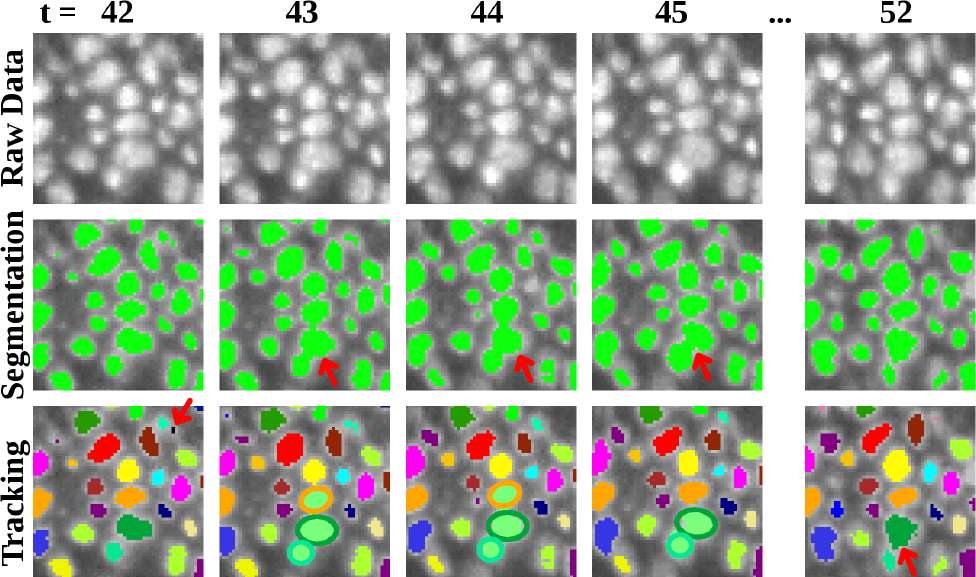
\includegraphics[width=\textwidth]{images/gmm/results/B/result_with_demerging.png}
    \caption[Excerpt of data set A: raw data, segmentation and tracking result]{A short time
        sequence of $2d$ images extracted from the $3d+t$ data set B of a drosophila embryo shortly
        after gastrulation~(taken from \citealp{schiegg_13_conservation}). The first row shows the raw
        data, followed by the segmentation in the middle row and, finally, the tracking result in
        the bottom row. Segmentation errors that stem from multiple objects being detected as a
        single connected component~(undersegmentation) are indicated by red arrows in the middle
        row. Moreover, the red arrow at $t=42$ in the bottom row shows an oversegmentation error that has been
        disabled by the tracking as indicated by black color. In the bottom row, the ellipses in
        time steps $43$-$45$ represent Gaussian mixture models that were fit to the detected merged
        connected components with the appropriate number of components. Our model is capable of
        reproducing the cell identities over a long time range ($42$-$52$), even if the merger
        configuration changes over time~(the addressed connected components contain three cells in
        time steps $43$ and $42$, and two cells at time $44$).}
    \label{fig:gmm-result-b}
\end{figure}
In the second data set B, the cell population is much denser compared to data set A. As a result,
the segmentation~\citep{sommer_11_ilastik} contains many merged
objects~(\cref{fig:gmm-result-b}). While these undersegmentation errors cannot be handled by
\citet{kausler_12_discrete}, our method makes use of its merger detection and cell reconstruction
capabilities~(\cref{tab:gmm-result-b}).

The tracking results are evaluated with respect to ground truth that has been generated
manually. \cref{tab:gmm-result-b} summarizes these results on data set B. Naturally,
\citep{kausler_12_discrete} cannot produce results for merged objects as they do not model multiple
objects per connected component. However, as shown in \cref{fig:gmm-result-b}, resolving merged
objects is vital for competitive tracking result in this data set. This is reflected by our method
outperforming the method in \citet{kausler_12_discrete}, \eg for divisions, they achieve an
$\fmeasure$-score of $0.06$ compared to our model's $0.71$. In addition to an accurate detection of
the correct number of objects in a connected component (precision$=0.78$), our model can resolve the
identities of these merged objects and reproduce moves over multiple frames with an
$\fmeasure$-score of $0.67$. Note that evaluation of multiframe moves is not conditioned on the
correct detections and transitions of mergers. Thus, an error in the detection of a merger will
automatically degrade the performance of the multiframe move reconstruction.

\begin{table}
    % \small
    % \hfill{}
    \centering
    \begin{tabular}{l||ccc|ccc}
        \toprule
        & \multicolumn{3}{c|}{\textbf{Moves}} & \multicolumn{3}{c}{\textbf{Divisions}}  \\
        & Precision & Recall & $F_1$& Precision& Recall& $F_{1}$\\
        \hline
        \citep{kausler_12_discrete} 	& 0.92		& 0.92 & 0.92  & 0.05      & 0.12 & 0.06    \\
        Classifiers only 	& \textit{N/A}	& \textit{N/A} & \textit{N/A}  & 0.83      & 0.64 & 0.72    \\
        Ours ($m=1$)						& 0.97        & 0.95 & 0.96  & 0.62     & 0.63 & 0.63    \\  
        Ours ($m=2$)						& 0.97        & 0.97 & 0.97  & 0.53      & 0.79 & 0.64   \\ 
        Ours ($m=3$)						& 0.97        & 0.97 & 0.97  & 0.70      & 0.76 & 0.73    \\ 
        Ours ($m=4$)						& 0.97        & 0.97 & 0.97  & 0.65      & 0.77 & 0.71    \\ 
        \midrule
        & \multicolumn{3}{c|}{\textbf{Mergers} } & \multicolumn{3}{c}{\textbf{Resolved Mergers}} \\
        & Precision& Recall& $F_{1}$ & Precision& Recall& $F_{1}$ \\
        \hline
        \citep{kausler_12_discrete} & \textit{N/A}& \textit{N/A} & \textit{N/A} & \textit{N/A}& \textit{N/A} & \textit{N/A} \\
        Classifiers only & 0.63 & 0.31 & 0.41 & \textit{N/A}& \textit{N/A} & \textit{N/A} \\
        Ours ($m=1$) & \textit{N/A}& \textit{N/A} & \textit{N/A} & \textit{N/A}& \textit{N/A} & \textit{N/A}\\
        Ours ($m=2$) & 0.71 & 0.54 & 0.61 & 0.72 & 0.61 & 0.66 \\
        Ours ($m=3$) & 0.73 & 0.58 & 0.64  & 0.73      & 0.63 & 0.67 \\
        Ours ($m=4$) & 0.78      & 0.59 & 0.67 & 0.74      & 0.63 & 0.60 \\
        \bottomrule
    \end{tabular}
    \caption[Conservation tracking results: Data Set B]{Evaluation of the performance on data set
        B~(taken and modified from \citealp[Table~2]{schiegg_13_conservation}). The tracking results
        are evaluated with regard to manually generated ground truth.}
    \label{tab:gmm-result-b}
\end{table}


Another building block for the success of our model on this data set is the use of the probabilistic
division prior $\phi_{\text{div}}$ that -- by itself -- reaches an $\fmeasure$-score of $0.72$ for
predicting mitotic cells. In order to give an overview of the tracking result and also to show the
complexity of cell tracking, \cref{fig:gmm-result-b-projection} shows a $2d$ projection of the $3d$
trajectories of cells in data set B.

\begin{figure}
    \centering
    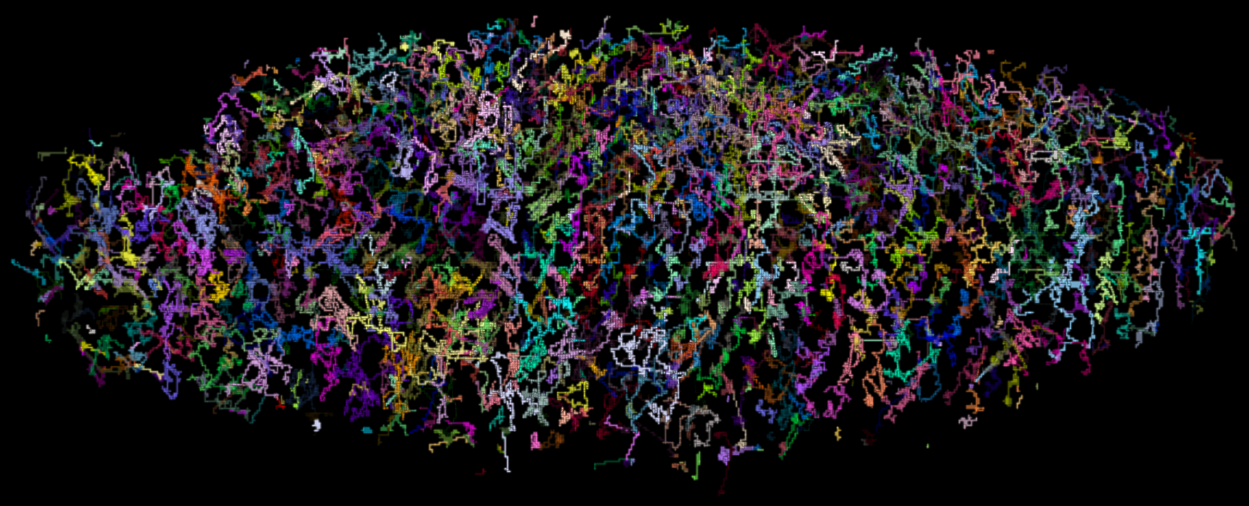
\includegraphics[width=\textwidth]{images/gmm/results/B/projection.png}
    \caption[$2d$ projection of trajectories in data set B]{$2d$ projection of the $3d$ trajectories of cells in data set B~(taken from
        \citealp{schiegg_13_conservation}): Colors encode individual cells. In case of divisions,
        both child cells take the color of their ancestor cell.}
    \label{fig:gmm-result-b-projection}
\end{figure}



\subsubsection{Data Set C - MitoCheck}
\def\imagetop#1{\vtop{\null\hbox{#1}}}
\newlength\tablemathtext
\settototalheight\tablemathtext{\parbox{\linewidth}{$t=75$, $\id=446$}}
\begin{table}
    \centering
    \scalebox{0.85}{
        \def\arraystretch{0.5}
% \setlength{\tabcolsep}{1pt}
\begin{tabular}{lccc}
    \toprule
    Time Step \& Id  & Raw Data & Segmentation & GMM fit \\ \midrule
    % \begin{minipage}[t]{0.15\linewidth}\small\vspace{-53pt}{$\begin{aligned}t&=75\\\id&=446\\
    %         k&=3\end{aligned}$}\end{minipage}&
    % \raisebox{-0.8\height{\includegraphics...}}
    $t=75$, $\id=446$&
    \raisebox{\tablemathtext-\height}{
        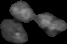
\includegraphics[width=0.18\textwidth]{images/gmm/gmm_2d_fit/t=75,id=446,k=3_raw.png}} &
    \raisebox{\tablemathtext-\height}{
        
\includegraphics[width=0.18\textwidth]{images/gmm/gmm_2d_fit/t=75,id=446,k=3_label.png}} &
    \raisebox{\tablemathtext-\height}{
        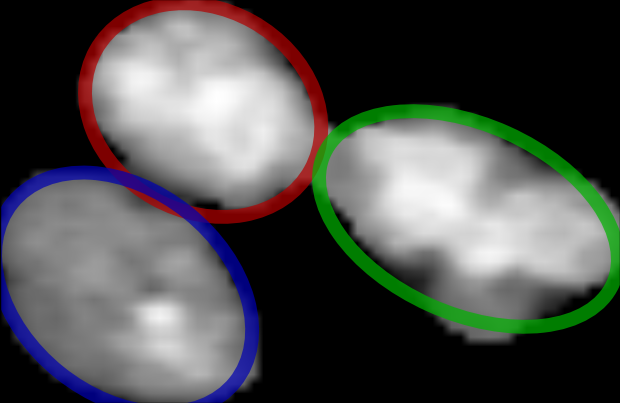
\includegraphics[width=0.18\textwidth]{images/gmm/gmm_2d_fit/t=75,id=446,k=3_fit.png}} \\
    &&& \\
    $t=85$, $\id=12$&
    \raisebox{\tablemathtext-\height}{
        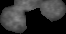
\includegraphics[width=0.18\textwidth]{images/gmm/gmm_2d_fit/t=85,id=12,k=3_raw.png}} &
    \raisebox{\tablemathtext-\height}{
        
\includegraphics[width=0.18\textwidth]{images/gmm/gmm_2d_fit/t=85,id=12,k=3_label.png}} &
    \raisebox{\tablemathtext-\height}{
        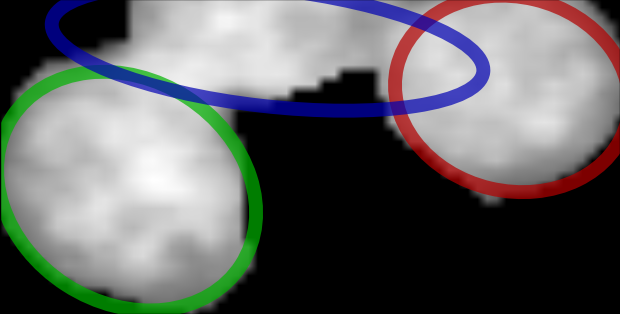
\includegraphics[width=0.18\textwidth]{images/gmm/gmm_2d_fit/t=85,id=12,k=3_fit.png}} \\
    &&& \\
    $t=75$, $\id=206$&
    \raisebox{\tablemathtext-\height}{
        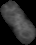
\includegraphics[width=0.18\textwidth]{images/gmm/gmm_2d_fit/t=75,id=206,k=2_raw.png}} &
    \raisebox{\tablemathtext-\height}{
        
\includegraphics[width=0.18\textwidth]{images/gmm/gmm_2d_fit/t=75,id=206,k=2_label.png}} &
    \raisebox{\tablemathtext-\height}{
        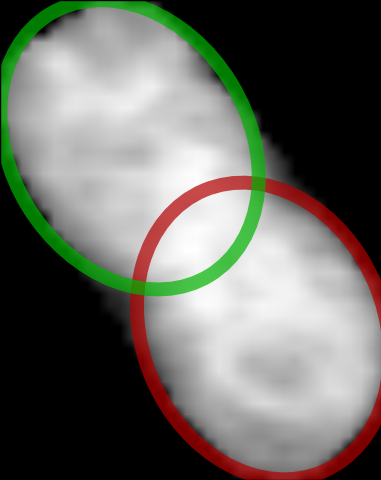
\includegraphics[width=0.18\textwidth]{images/gmm/gmm_2d_fit/t=75,id=206,k=2_fit.png}} \\
    % &
    % \raisebox{\tablemathtext-\height}{
\includegraphics[width=0.18\textwidth]{images/gmm/gmm_2d_fit/t=50,id=198,k=3_raw.png}} &
    % \raisebox{\tablemathtext-\height}{
\includegraphics[width=0.18\textwidth]{images/gmm/gmm_2d_fit/t=50,id=198,k=3_label.png}} &
    % \raisebox{\tablemathtext-\height}{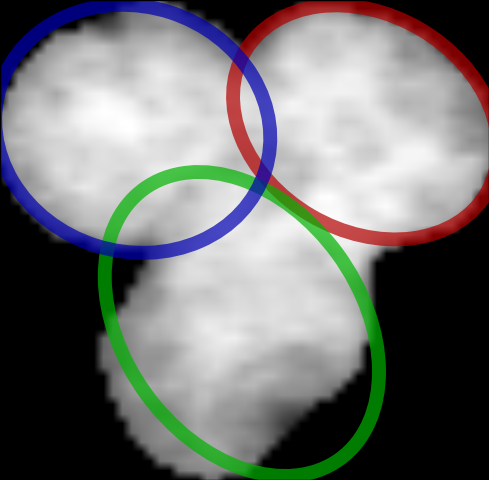
\includegraphics[width=0.18\textwidth]{images/gmm/gmm_2d_fit/t=50,id=198,k=3_fit.png}} \\ &
    &&& \\
    $t=75$, $\id=446$&
    \raisebox{\tablemathtext-\height}{
        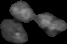
\includegraphics[width=0.18\textwidth]{images/gmm/gmm_2d_fit/t=75,id=446,k=3_raw.png}} &
    \raisebox{\tablemathtext-\height}{
\includegraphics[width=0.18\textwidth]{images/gmm/gmm_2d_fit/t=75,id=446,k=3_label.png}} &
    \raisebox{\tablemathtext-\height}{
        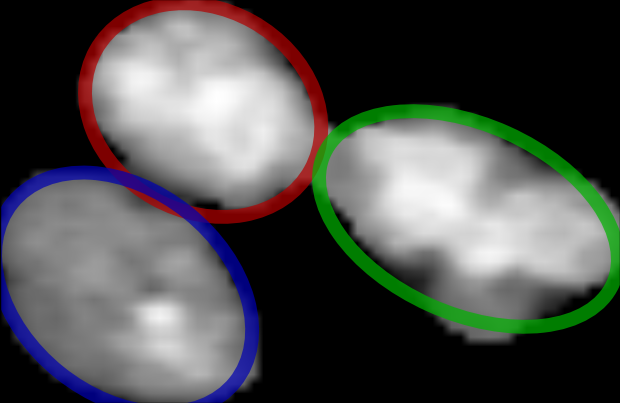
\includegraphics[width=0.18\textwidth]{images/gmm/gmm_2d_fit/t=75,id=446,k=3_fit.png}} \\
    &&& \\
    $t=50$, $\id=122$&
    \raisebox{\tablemathtext-\height}{
        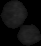
\includegraphics[width=0.18\textwidth]{images/gmm/gmm_2d_fit/t=50,id=122,k=2_raw.png}} &
    \raisebox{\tablemathtext-\height}{
\includegraphics[width=0.18\textwidth]{images/gmm/gmm_2d_fit/t=50,id=122,k=2_label.png}} &
    \raisebox{\tablemathtext-\height}{
        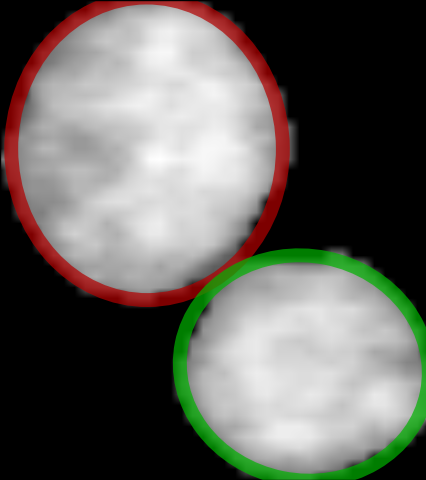
\includegraphics[width=0.18\textwidth]{images/gmm/gmm_2d_fit/t=50,id=122,k=2_fit.png}} \\
    &&& \\
    $t=85$, $\id=334$&
    \raisebox{\tablemathtext-\height}{
        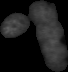
\includegraphics[width=0.18\textwidth]{images/gmm/gmm_2d_fit/t=85,id=334,k=4_raw.png}} &
    \raisebox{\tablemathtext-\height}{
        \hspace{-3pt}
\includegraphics[width=0.18\textwidth]{images/gmm/gmm_2d_fit/t=85,id=334,k=4_label.png}} &
    \raisebox{\tablemathtext-\height}{
        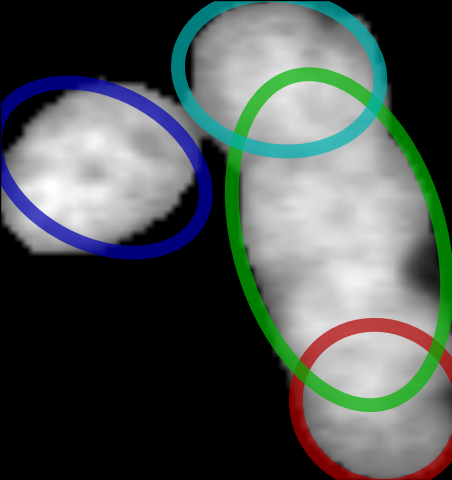
\includegraphics[width=0.18\textwidth]{images/gmm/gmm_2d_fit/t=85,id=334,k=4_fit.png}} \\
    \bottomrule
\end{tabular}
\def\arraystretch{1.0}

% WHY THE FUCK THE NEED FOR NEGATIVE HSPACE IN LAST ROW?

%%% Local Variables: 
%%% mode: latex
%%% TeX-master: "../../../../main"
%%% End: 

    }
    \caption[GMM fits to two-dimensional cells]{\small GMM fits to two-dimensional cells from data set
        C: Based on the inferred number of cells per connected components, the rightmost column
        shows GMM fits to the bounding box images of merged objects with ids $\id$ at times $t$ as an overlay
        on the raw data. Here, the ellipses represent covariances of mixture components, centered
        add the corresponding means. Note that
        column two shows the connected components in their original intensity range, whereas the intensity
        has been stretched to $[0,255]$ in the rightmost column in the process of overlaying the
        fit. Furthermore, partial objects in the segmentation, which are not objects of interest, are not
        displayed. The second row shows a merged object that has been cut off by the image border. Still,
        conservation tracking manages to infer the correct number of cells and the GMM fit yields a
        reasonable estimate on the region centers of the individual objects.}
   \label{tab:gmm-results-c-fits}
\end{table}

Data set C completes our evaluation of the model. Again, a gold standard for evaluation has been
acquired manually. Other than the data sets above, data set C has only two spatial dimensions, which
necessarily leads to merged objects caused by occlusion, even if the image quality is
good~(\cref{fig:gmm-data-c-three-slices,tab:gmm-results-c-fits}). This time, the merger classifiers
perform weakly, but the conservation tracking graphical model boosts this result. In general, with
an active merger detection, \ie $m>1$, our approach outperforms the method of
\citet{kausler_12_discrete}. \cref{tab:gmm-result-c} summarizes the results for four different
settings of the parameter $m$, which specifies the maximum possible number of objects per connected
component.
%In addition, \cref{tab:gmm-number-of-merged-objects} shows the number of merged objects
%inferred by our method for both data set B and data set C.

\begin{table} % \small % \hfill{} \centering
    \begin{tabular}{l||ccc|ccc}
        \toprule
        & \multicolumn{3}{c|}{\textbf{Moves}} & \multicolumn{3}{c}{\textbf{Divisions}} \\
        & Precision& Recall& $\fmeasure$ & Precision& Recall& $\fmeasure$ \\ \hline
        \citep{kausler_12_discrete} & 0.99 & 0.97 & 0.98 & 0.65 & 0.68 & 0.66 \\
        Classifiers only & \textit{N/A} & \textit{N/A} & \textit{N/A} & 0.92 & 0.56 & 0.70 \\
        Ours ($m=1$) & 0.99 & 0.97 & 0.98 & 0.68 & 0.71 & 0.70 \\
        Ours ($m=2$) & 1.00 & 0.99 & 0.99 & 0.85 & 0.76 & 0.80 \\
        Ours ($m=3$) & 1.00 & 0.99 & 0.99 & 0.85 & 0.77 & 0.80 \\
        Ours ($m=4$) & 1.00 & 0.99 & 0.99 & 0.85 & 0.76 & 0.80 \\
        \midrule & \multicolumn{3}{c|}{\textbf{Mergers} } & \multicolumn{3}{c}{\textbf{Resolved Mergers}} \\ 
        & Precision& Recall& $F_{1}$ & Precision& Recall& $F_{1}$ \\ \hline
        \citet{kausler_12_discrete} & \textit{N/A}& \textit{N/A} & \textit{N/A} & \textit{N/A}&
        \textit{N/A} & \textit{N/A} \\
        Classifiers only & 0.41 & 0.62 & 0.49 & \textit{N/A}& \textit{N/A} & \textit{N/A} \\
        Ours ($m=1$) & \textit{N/A}& \textit{N/A} & \textit{N/A} & \textit{N/A}& \textit{N/A} & \textit{N/A}\\ 
        Ours ($m=2$) & 0.73 & 0.60 & 0.66 & 0.79 & 0.70 & 0.74\\
        Ours ($m=3$) & 0.84 & 0.69 & 0.76 & 0.85 & 0.75 & 0.79\\
        Ours ($m=4$) & 0.84 & 0.69 & 0.76 & 0.85 & 0.75 & 0.80\\
        \bottomrule
    \end{tabular}
    \caption[Conservation tracking results: Data Set C]{Evaluation of the performance on data set
C~(taken and modified from \citealp[Table~2]{schiegg_13_conservation}). The tracking results are
evaluated with regard to manually generated ground truth.}
    \label{tab:gmm-result-c}
\end{table}


Again, the set of optimal parameters as shown in \cref{tab:gmm-experiments-parameters} has been
determined by a grid search over a range of 720 parameters, which also allows for an evaluation of
the sensitivity to parameter changes of our model. To that end, \cref{fig:gmm-results-c-vis-sensitivity}
plots the $\fmeasure$ performances for each parameter setting. Naturally, with a high number of
unambiguous moves in data set C, the overall $\fmeasure$-score is not affected by the choice of
parameters. Even though there are a couple of outlier parameter settings that perform badly for
divisions, the method is fairly robust to variation of the parameter settings.
% \begin{table}
%     \centering
%     \begin{tabular}{l||ccc|ccc}
%         \toprule
%         &\multicolumn{3}{c|}{\textbf{Data Set B}}&\multicolumn{3}{c}{\textbf{Data Set B}} \\
%         & $(2)$ & $(3)$ & $(4)$ & $(2)$ & $(3)$ & $(4)$ \\ \hline
%         Ours $(m=2)$ & 979 & \textit{N/A} & \textit{N/A} &&& \\
%         Ours $(m=3)$ & 859 & 116 & \textit{N/A} &&& \\
%         Ours $(m=4)$ & 859 & 115 & 1 &&& \\
%         Ground Truth & 987 & 156 & 48 &&& \\
%         \bottomrule
%     \end{tabular}
%     \caption{Number of merged objects per connected component in data sets B and C.}
%     \label{tab:gmm-number-of-merged-objects}
% \end{table}
\begin{figure}
    \centering
    \begin{subfigure}[t]{0.48\textwidth}
        \centering
        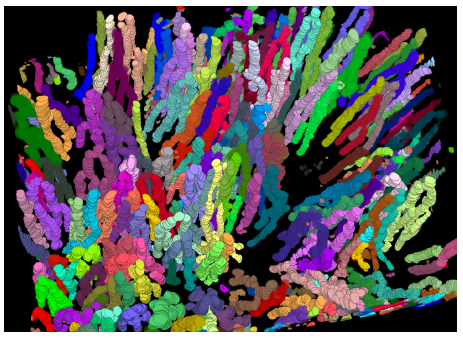
\includegraphics[width=\textwidth]{images/gmm/results/C/space_time_rendering.png}
        \caption{Space-time rendering of the conservation tracking result~(taken from
            \citealp[Figure~6c]{schiegg_13_conservation}).}
        \label{fig:gmm-results-c-visualization}
    \end{subfigure}
    \hfill
    \begin{subfigure}[t]{0.48\textwidth}
        \centering
        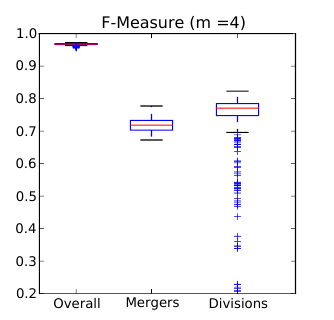
\includegraphics[width=0.828\textwidth]{images/gmm/results/C/sensitivity.png}
        \caption{Parameter sensitivity of the $\fmeasure$ performance on the overall tracking as
            well as on merger and division events for our method on data set C~(taken from
            \citealp[Figure~6d]{schiegg_13_conservation}).}
        \label{fig:gmm-results-c-sensitivity}
    \end{subfigure}
    \caption[Visualization of the tracking results for data set C and parameter sensitivity]{The
        tracking result of our method is visualized in~(\subref{fig:gmm-results-c-visualization}) in
        terms of a space-time rendering the trajectories of the cells with each color indicating a
        unique track. Children cells inherit the color of their ancestor and divisions are clearly
        visible as forks of tracks into two branches of the same color. The parameter
        sensitivity evaluation (\subref{fig:gmm-results-c-sensitivity}) shows that our method is
        fairly robust towards a change in parameter settings.}
    \label{fig:gmm-results-c-vis-sensitivity}
\end{figure}




Finally, the results of the classifier evaluation in \cref{tab:gmm-result-c} show that global
information embedded in a graphical model give a strong boost to the comparibly weak performance of
the local merger classifiers.

In this chapter we introduced a cell reconstruction method for conservation tracking based on
Gaussian mixture models. In the experimental evaluation, conservation tracking performs comparably to
the state of the art method, chain graph tracking~(\cref{subsec:fg-chaingraph}), in a merger-free
setting. Furthermore, conservation tracking is able to reliably detect merged objects and
reconstruct unique tracks. Still, tracking results are highly dependent on the segmentation. To
address this, we present a joint segmentation and tracking method in \cref{cha:joint}, which breaks
the barrier between segmentation and tracking in the context of tracking-by-assignment.

% After the extensive discussion of our proposed model for cell identity reconstruction in the context
% of the conersvation tracking, both in theory and experiments, the following ~\cref{cha:joint} will
% be dedicated to the introduction of a new graphical model based method which breaks the barrier
% between segmentation and tracking.



%%% Local Variables: 
%%% mode: latex
%%% TeX-master: "../../../main"
%%% End: 
